\begin{figure}[H]
    \centering
    \begin{subfigure}{0.3\textwidth}
        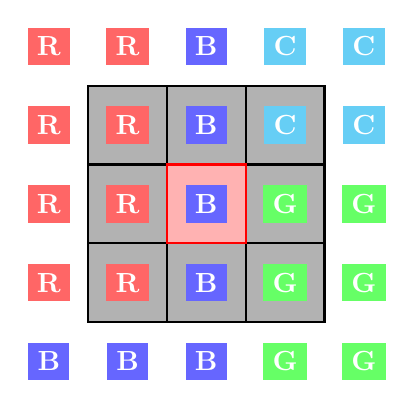
\begin{tikzpicture}

    \fill[black!30] (1, 4) rectangle ++(1,1);
    \fill[black!30] (3, 4) rectangle ++(1,1);
    \fill[black!30] (2, 3) rectangle ++(1,1);
    \fill[black!30] (2, 5) rectangle ++(1,1);
    \fill[black!30] (3, 5) rectangle ++(1,1);
    \fill[black!30] (3, 3) rectangle ++(1,1);
    \fill[black!30] (1, 5) rectangle ++(1,1);
    \fill[black!30] (1, 3) rectangle ++(1,1);

    \fill[red!30] (2, 4) rectangle ++(1,1);

    \draw[thick, black] (1, 4) rectangle ++(1,1);
    \draw[thick, black] (3, 4) rectangle ++(1,1);
    \draw[thick, black] (2, 3) rectangle ++(1,1);
    \draw[thick, black] (2, 5) rectangle ++(1,1);
    \draw[thick, black] (3, 5) rectangle ++(1,1);
    \draw[thick, black] (3, 3) rectangle ++(1,1);
    \draw[thick, black] (1, 5) rectangle ++(1,1);
    \draw[thick, black] (1, 3) rectangle ++(1,1);

    \draw[thick, red] (2, 4) rectangle ++(1,1);
    
    % Draw the grid and add colored letters
    \node[fill=red!60, text=white, font=\bfseries] at (0.5, 6.5) {R}; 
    \node[fill=red!60, text=white, font=\bfseries] at (1.5, 6.5) {R}; 
    \node[fill=blue!60, text=white, font=\bfseries] at (2.5, 6.5) {B}; 
    \node[fill=cyan!60, text=white, font=\bfseries] at (3.5, 6.5) {C}; 
    \node[fill=cyan!60, text=white, font=\bfseries] at (4.5, 6.5) {C};
    
    \node[fill=red!60, text=white, font=\bfseries] at (0.5, 5.5) {R}; 
    \node[fill=red!60, text=white, font=\bfseries] at (1.5, 5.5) {R}; 
    \node[fill=blue!60, text=white, font=\bfseries] at (2.5, 5.5) {B}; 
    \node[fill=cyan!60, text=white, font=\bfseries] at (3.5, 5.5) {C}; 
    \node[fill=cyan!60, text=white, font=\bfseries] at (4.5, 5.5) {C};
    
    \node[fill=red!60, text=white, font=\bfseries] at (0.5, 4.5) {R}; 
    \node[fill=red!60, text=white, font=\bfseries] at (1.5, 4.5) {R}; 
    \node[fill=blue!60, text=white, font=\bfseries] at (2.5, 4.5) {B};  % Nodo centrale
    \node[fill=green!60, text=white, font=\bfseries] at (3.5, 4.5) {G}; 
    \node[fill=green!60, text=white, font=\bfseries] at (4.5, 4.5) {G};
    
    \node[fill=red!60, text=white, font=\bfseries] at (0.5, 3.5) {R}; 
    \node[fill=red!60, text=white, font=\bfseries] at (1.5, 3.5) {R}; 
    \node[fill=blue!60, text=white, font=\bfseries] at (2.5, 3.5) {B}; % Vicino dello stesso colore
    \node[fill=green!60, text=white, font=\bfseries] at (3.5, 3.5) {G}; 
    \node[fill=green!60, text=white, font=\bfseries] at (4.5, 3.5) {G};
    
    \node[fill=blue!60, text=white, font=\bfseries] at (0.5, 2.5) {B}; 
    \node[fill=blue!60, text=white, font=\bfseries] at (1.5, 2.5) {B}; % Vicino dello stesso colore
    \node[fill=blue!60, text=white, font=\bfseries] at (2.5, 2.5) {B}; % Vicino dello stesso colore
    \node[fill=green!60, text=white, font=\bfseries] at (3.5, 2.5) {G}; 
    \node[fill=green!60, text=white, font=\bfseries] at (4.5, 2.5) {G};
\end{tikzpicture}
        \caption{Il nodo centrale "B" è colorato in giallo con un bordo rosso, mentre i nodi vicini dello stesso colore sono colorati in magenta.}
    \end{subfigure}
    \hfill
    \begin{subfigure}{0.3\textwidth}
        \input{tikz/tikzpicture2.tikz}
        \caption{Il nodo centrale "B" è colorato in giallo con un bordo rosso, mentre i nodi vicini dello stesso colore sono colorati in magenta.}
    \end{subfigure}
    \hfill
    \begin{subfigure}{0.3\textwidth}
        \input{tikz/tikzpicture3.tikz}
        \caption{Il nodo centrale "B" è colorato in giallo con un bordo rosso, mentre i nodi vicini dello stesso colore sono colorati in magenta.}
    \end{subfigure}

    \vspace{20pt}
    \begin{subfigure}{0.3\textwidth}
        \input{tikz/tikzpicture4.tikz}
        \caption{Il nodo centrale "B" è colorato in giallo con un bordo rosso, mentre i nodi vicini dello stesso colore sono colorati in magenta.}
    \end{subfigure}
    \hfill
    \begin{subfigure}{0.3\textwidth}
        \input{tikz/tikzpicture5.tikz}
        \caption{Il nodo centrale "B" è colorato in giallo con un bordo rosso, mentre i nodi vicini dello stesso colore sono colorati in magenta.}
    \end{subfigure}
    \hfill
    \begin{subfigure}{0.3\textwidth}
        \input{tikz/tikzpicture6.tikz}
        \caption{Il nodo centrale "B" è colorato in giallo con un bordo rosso, mentre i nodi vicini dello stesso colore sono colorati in magenta.}
    \end{subfigure}
\end{figure}